\documentclass[12pt,a4paper,twoside]{article}
\usepackage{labor}
\begin{document}

%fill for cover and header creation
\newcommand\laboratorynumber{2}
\title{Fallrohr}
\newcommand\supervisor{Ditlbacher, Harald}
\newcommand\groupnumber{42}

\newcommand\participantonelastname{Eisner}
\newcommand\participantonefirstname{Nico}
\newcommand\participantoneid{12214121}
\newcommand\participanttwolastname{Waldl}
\newcommand\participanttwofirstname{Philip}
\newcommand\participanttwoid{12214120}
\author{\participantonelastname \ \& \participanttwolastname}

\newcommand\degreeid{UB 033 678}
\newcommand\semester{23WS}
\date{11.11.2023}

%select correct course title
%\newcommand\coursetitle{Einführung in die \\ physikalischen Messmethoden}
%\newcommand\coursetitle{Laborübungen 1: \\ Mechanik und Wärme}
\newcommand\coursetitle{Laborübungen 2: \\ Elektrizität, Magnetismus, Optik}
%\newcommand\coursetitle{Fortgeschrittenen Praktikum 1: \\ Technische Physik}
%\newcommand\coursetitle{Fortgeschrittenen Praktikum 2: \\ Allgemeine Physik}

%\begin{titlepage}
   \begin{center}
       \begin{figure}[H]
            \begin{minipage}[h]{30mm}
                \centerline{
\includegraphics[height=15mm]{cover_nudes/tugraz.png}}
            \end{minipage}
            \hfill
            \begin{minipage}[h]{30mm}
                \centerline{
\includegraphics[height=15mm]{cover_nudes/nawi_graz.png}}
            \end{minipage}
            \hfill
            \begin{minipage}[h]{30mm}
                \centerline{
\includegraphics[height=15mm]{cover_nudes/uni-graz.png}}
            \end{minipage}
        \end{figure}
        
        \large{\emph{Institut für Experimentalphysik der Technischen Universität Graz \\
        \& Institut für Physik der Universität Graz}} \\
        \vspace{5mm}
        
        {\Huge \textbf{\coursetitle}}
        \vspace{5mm}
        
        {\huge \laboratorynumber: \thetitle}
    \end{center}
    
    \vfill
    
    \begin{table}[H]
        \LARGE
        \centering
        \begin{tabular}{r l}
            Betreuer:       & \supervisor \\
            Gruppennummer:  & \groupnumber \\
            \\
            Name:           & \participantonelastname, \participantonefirstname \\
            Matrikelnummer: & \participantoneid \\
            Name:           & \participanttwolastname, \participanttwofirstname \\
            Matrikelnummer: & \participanttwoid \\
            \\
            Kennzahl:       & \degreeid \\
            Datum:          & \semester \ | \thedate
        \end{tabular}
    \end{table}
    \vspace{4cm}
\end{titlepage}
\clearpage
\setcounter{page}{1}

%\maketitle %short title alternative


\includepdf[pages={1}]{../Deckblätter/Deckblatt_Transformator.pdf}

\tableofcontents
\newpage

\section{Aufgabenstellung} %jo beschreibn wos gmocht host ------------------------------
Der Versuch Transformator / Hysterese behandelt, wie aus dem Namen bereits hervorgeht, den Funktionsbereich des Transformators, in welchem in erster Linie die Umwandlung von elektsichen Spannungen hineinfällt.
Anhand von einer elektrischen Schaltung, welche im weiteren Verlauf des Experimentes immer wieder erweitert wird, soll die Rolle des Transformators veranschaulicht werden.
Zu erledigen war dabei folgender Versuchsauftrag:

\begin{itemize}
    \item Schaltung im Leerlauf
    \begin{itemize}
        \item Primärstrom $I_{1}$
        \item Primärspannung $U_{1}$
        \item Wirkleistung $P_{1}$
        \item Sekundärspannung $U_{2}$
        \item Sekundärstrom $I_{2}$
        \item Oszillographische Darstellung von Primärstrom und Sekundärspannung
    \end{itemize}
    \item Schaltung mit Ohm'scher Last sekundärseitig
    \begin{itemize}
        \item Primärstrom $I_{1}$
        \item Primärspannung $U_{1}$
        \item Wirkleistung $P_{1}$
        \item Sekundärspannung $U_{2}$
        \item Sekundärstrom $I_{2}$
        \item Oszillographische Darstellung von Primärstrom und Sekundärspannung
    \end{itemize}
    \item Schaltung mit Ohm'sch-induktiver Last (für ca. 20 Widerstandswerte)
    \begin{itemize}
        \item Primärstrom $I_{1}$
        \item Primärspannung $U_{1}$
        \item Wirkleistung $P_{1}$
        \item Sekundärspannung $U_{2}$
        \item Sekundärstrom $I_{2}$
        \item Oszillographische Darstellung der Sekundärspannung an der Stelle mit der größten Wirkleistung
    \end{itemize}
    \item \sout{Schaltung mit Ohm'sch-kapazitiver Last}
    \item Unsicherheitsberechnung für alle Punkte
\end{itemize}

\noindent
Alle Informationen und Methodiken wurden uns von der Technischen Universität bereitgestellt \cite{teachcenter1}. 


\section{Voraussetzungen \& Grundlagen} %Grundlagen erklären, Formeln mit erklärung

Wie im vorherigen Kapitel bereits eingeleitet dient ein Transformator dazu, von einer elektrischen Spannung auf eine andere zu transformieren. Im Aufbau sieht er dabei vereinfacht so aus:

\begin{figure}[H]
    \centering
    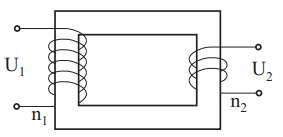
\includegraphics[width=0.5\linewidth]{nudes/GL-TrafoAufbau.png}
    \caption{Grundlegender Aufbau eines Transformators \cite{teachcenter1}}
    \label{fig:Aufbau Transformator}
\end{figure}

\noindent
Wie sich in Abbildung \ref{fig:Aufbau Transformator} erkennen lässt, besteht der Transformator aus zwei Spulen, welche über einen Eisenjoch miteinander verbunden sind. Die Umwandlung der Spannungen basiert auf dem Faraday'schen Gesetz

    \begin{equation}
        \label{eq:Faraday'sches Gesetz}
        \centerline{$U_{ind}=-N_{ind}\frac{d \phi}{dt}$}
    \end{equation}

\noindent
Wenn an der Primärspule eine Wechselspannung angelegt wird, wird ein sich änderndes (aufgrund der Richtungsänderung der Wechselspannung) Magnetfeld an der Primärspule (Eingangsspule) erzeugt. Durch dieses Magnetfeld wird an der Sekundärspule gemäß \ref{eq:Faraday'sches Gesetz} eine Ausgangsspannung induziert. 
Die resultierende Spannung ist dabei abhängig vom Wicklungsverhältnis der Spulen, was sich mit dem Ausdruck

\begin{equation}
    \label{eq:Verhältnis Wicklungen/Spannung}
    \centerline{$\frac{U2}{U1}=-\frac{n2}{n1}$}
\end{equation}

\noindent
beschreiben lässt. Der magnetische Fluss $\Phi$ setzt socj weiters in folgender Form zusammen:

\begin{equation}
    \label{eq:Magnetischer Fluss}
    \centerline{$\Phi = BA = \mu \mu_{0} HA = \mu \mu_{0} \frac{A}{l} nI$}
\end{equation}

\noindent
Sollte die Magnetisierungskurve $\Phi = \Phi(t)$ eine Hysterese, also eine verzögerte Entmagnetisierung von Ferromagnetischen Stoffen, aufweisen, so wird dem System Leistung entzogen und der Stromverlauf sieht wie folgt aus:

\begin{figure}[H]
    \centering
    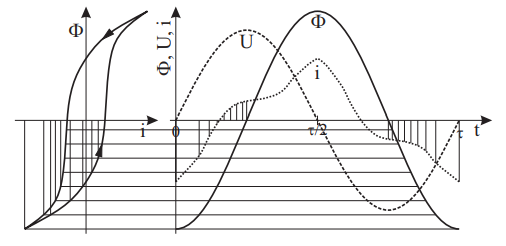
\includegraphics[width=0.5\linewidth]{nudes/GL-Hysterese.png}
    \caption{Magentischer Fluss mit Hysterese}
    \label{fig:Hystere}
\end{figure}

\noindent
Die Fläche innerhalb der in Abbildung \ref{fig:Hystere} gezeigten Hystereseschleife gibt Auskunft über die Hystereseverluste, welche gemeinsam mit den Wirbelstromverlusten die Eisenverluste am Trafo ergeben. \newline

\noindent
Zur Berechnung der Wirkleistung wird außerdem der Zusammenhang

\begin{equation}
    \label{eq:Wirkleistung}
    \centerline{$P_{W} = U*I$}
\end{equation}

\noindent
benötigt.


\section{Versuchsanordnung} %mit skizze kurz beschreiben ------------------------------

Das Herzstück des Versuches ist natürlich der Trafo, wobei bei diesem Experiment gleich zwei zum Einsatz kommen. Der gesamte Versuch basiert auf einer Grundschaltung, welche mit jedem Aufgabenpunkt ein wenig erweitert wird.

    \begin{figure}[H]
        \centering
        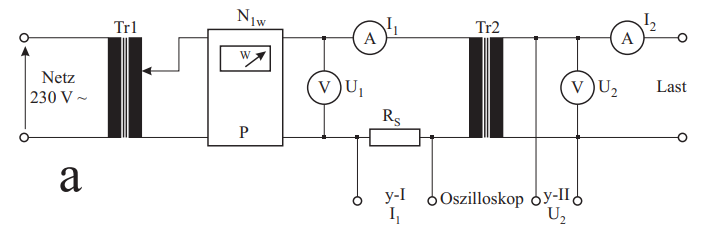
\includegraphics[width=0.6\linewidth, angle=0]{nudes/Versuchsaufbau a.png}
        \caption{Aufbau der Grundschaltung}
        \label{fig:AufbauDerGrundschaltung}
    \end{figure}

\noindent
In der Realität sieht der Aufbau wie folgt aus:

\begin{figure}[H]
    \centering
    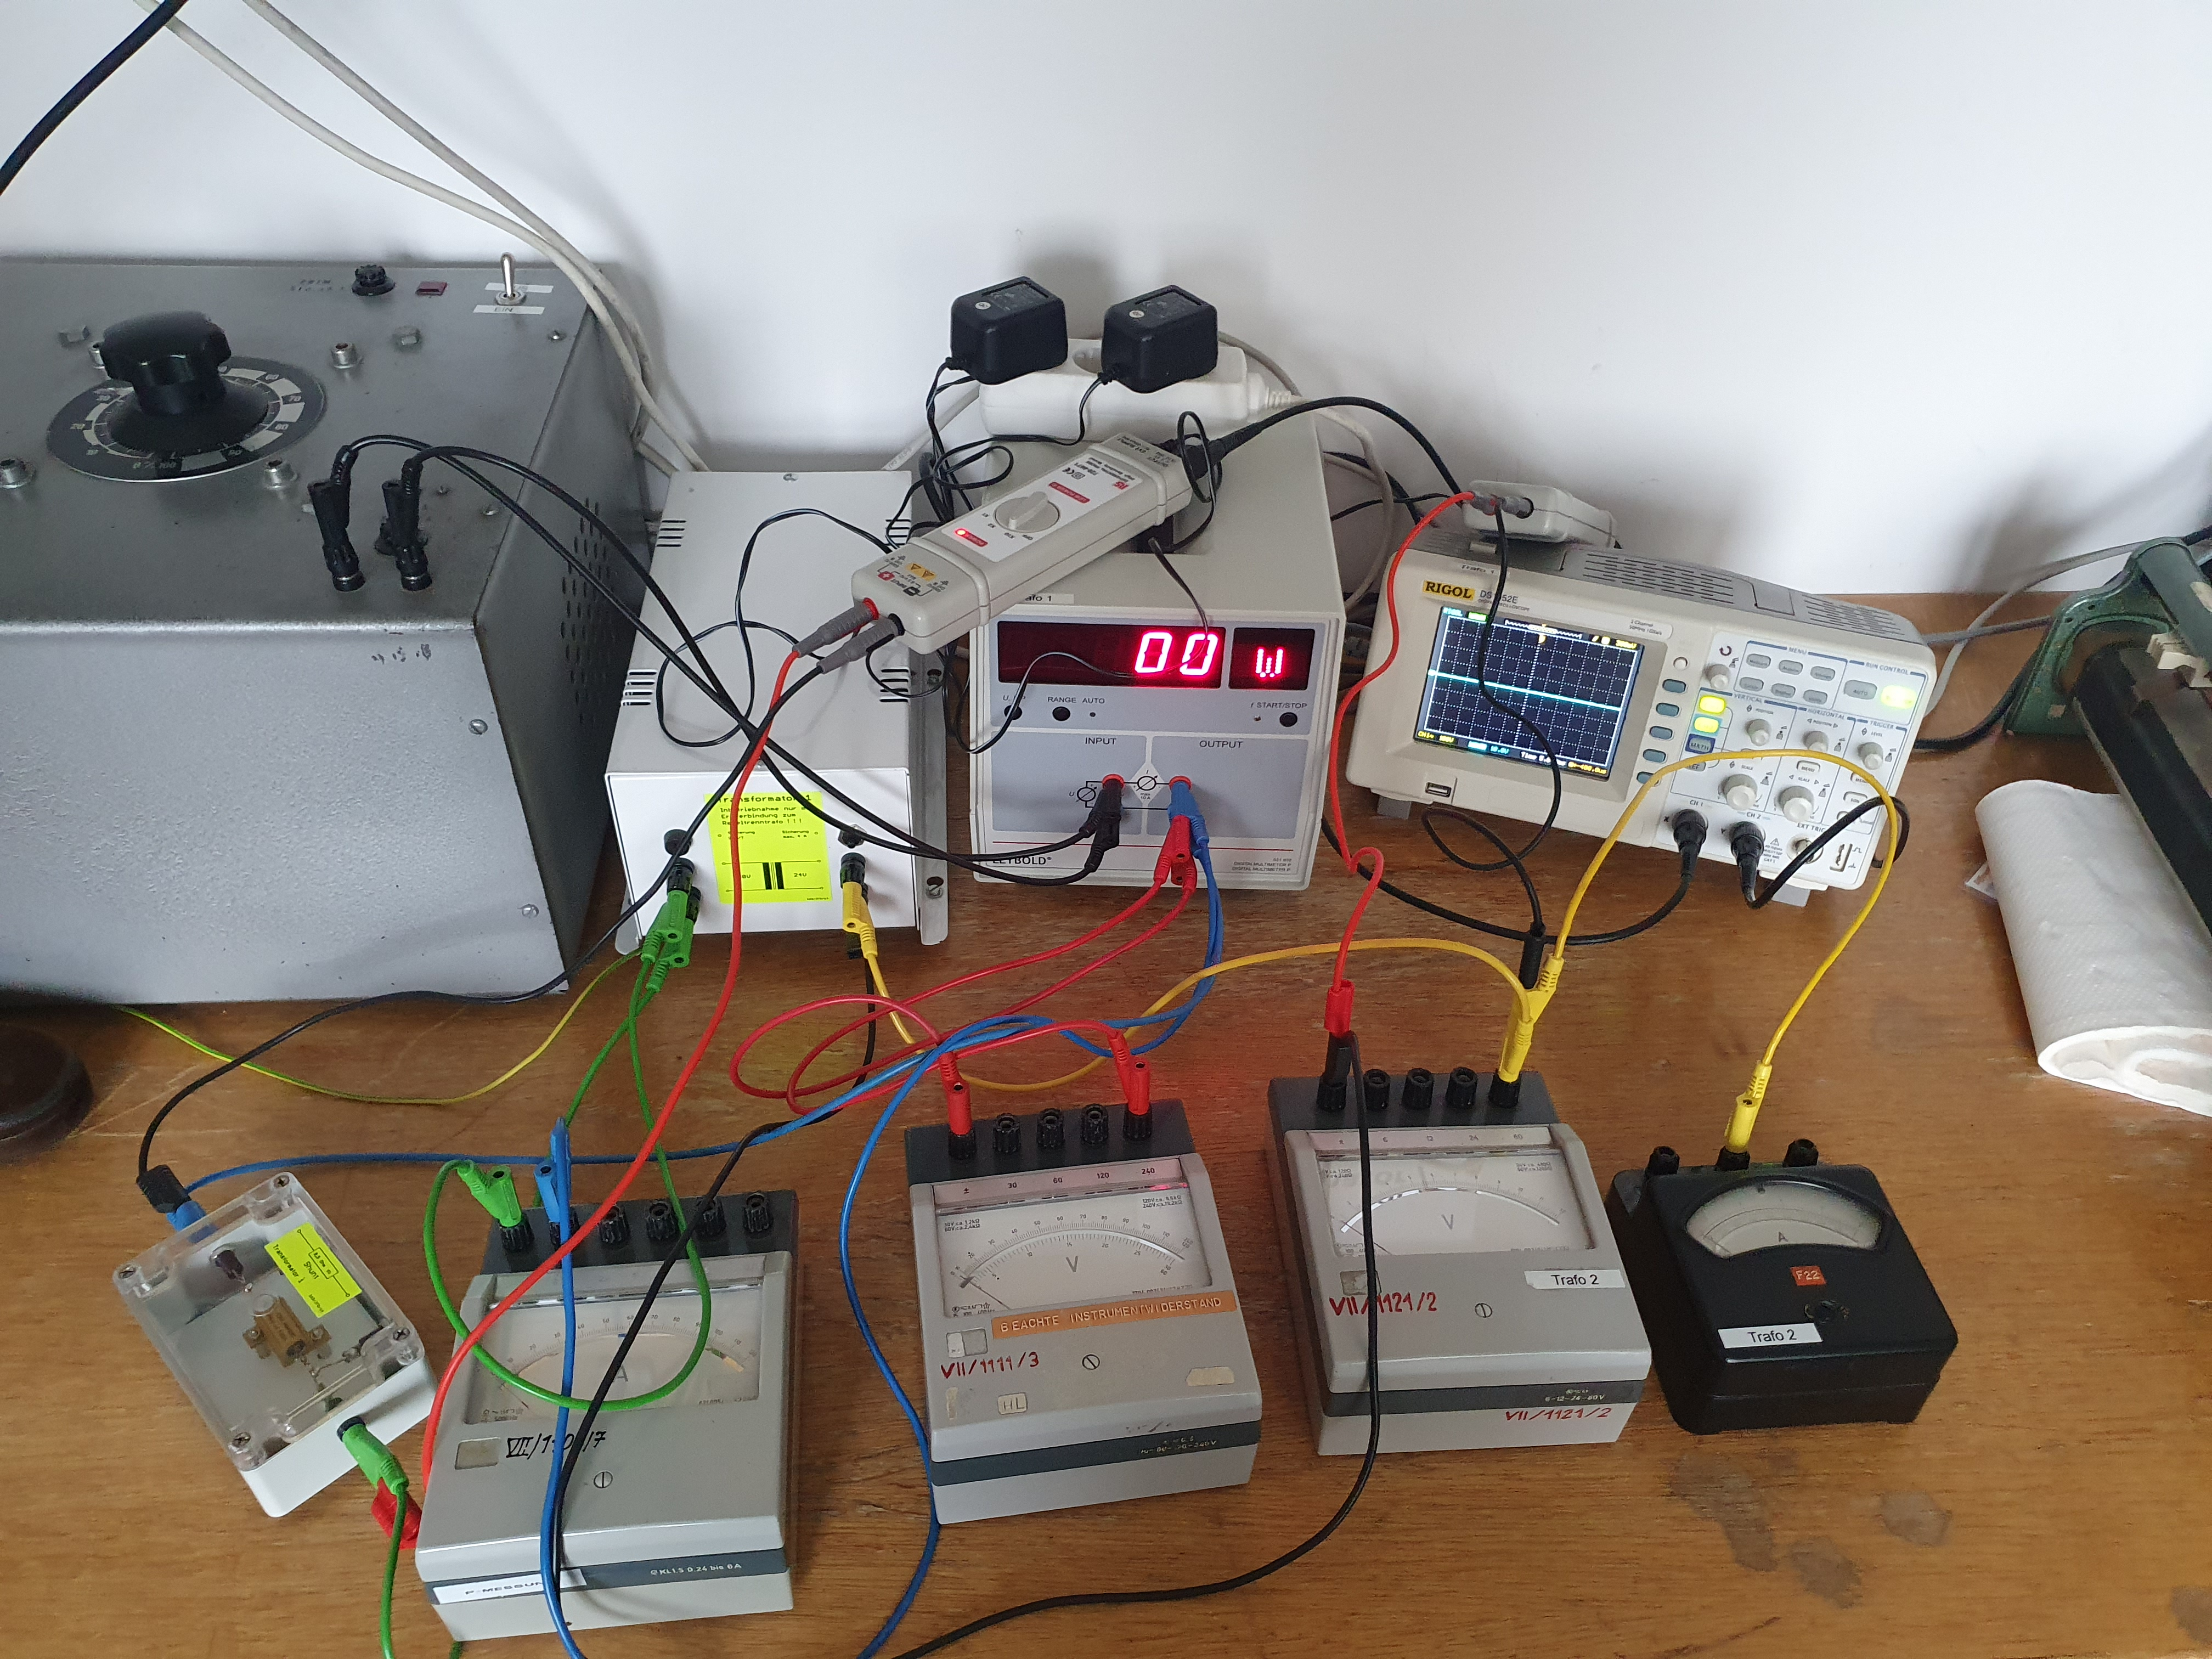
\includegraphics[width=0.6\linewidth, angle=0]{nudes/Aufbau a.png}
    \caption{Realer Aufbau der Grundschaltung}
    \label{fig:RealerAufbauDerGrundschaltung}
\end{figure}

\noindent
Im weiteren Verlauf des Experimentes wurde die Schaltung nicht wie in Abbildung \ref{fig:RealerAufbauDerGrundschaltung} im Leerlauf, sondern mit einem Lastwiderstand $R_{L}$ betrieben. Dadurch konnte nun auch ein Verbraucherstrom $I_{2}$ gemessen werden. Aufgebaut sieht der Versuch nun so aus:

\begin{figure}[H]
    \centering
    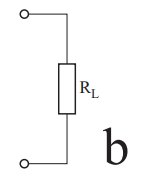
\includegraphics[width=0.2\linewidth, angle=0]{nudes/Versuchsaufbau b.png}
    \caption{Hinzugefügter Lastwiderstand}
    \label{fig:AufbauB}
\end{figure}

\begin{figure}[H]
    \centering
    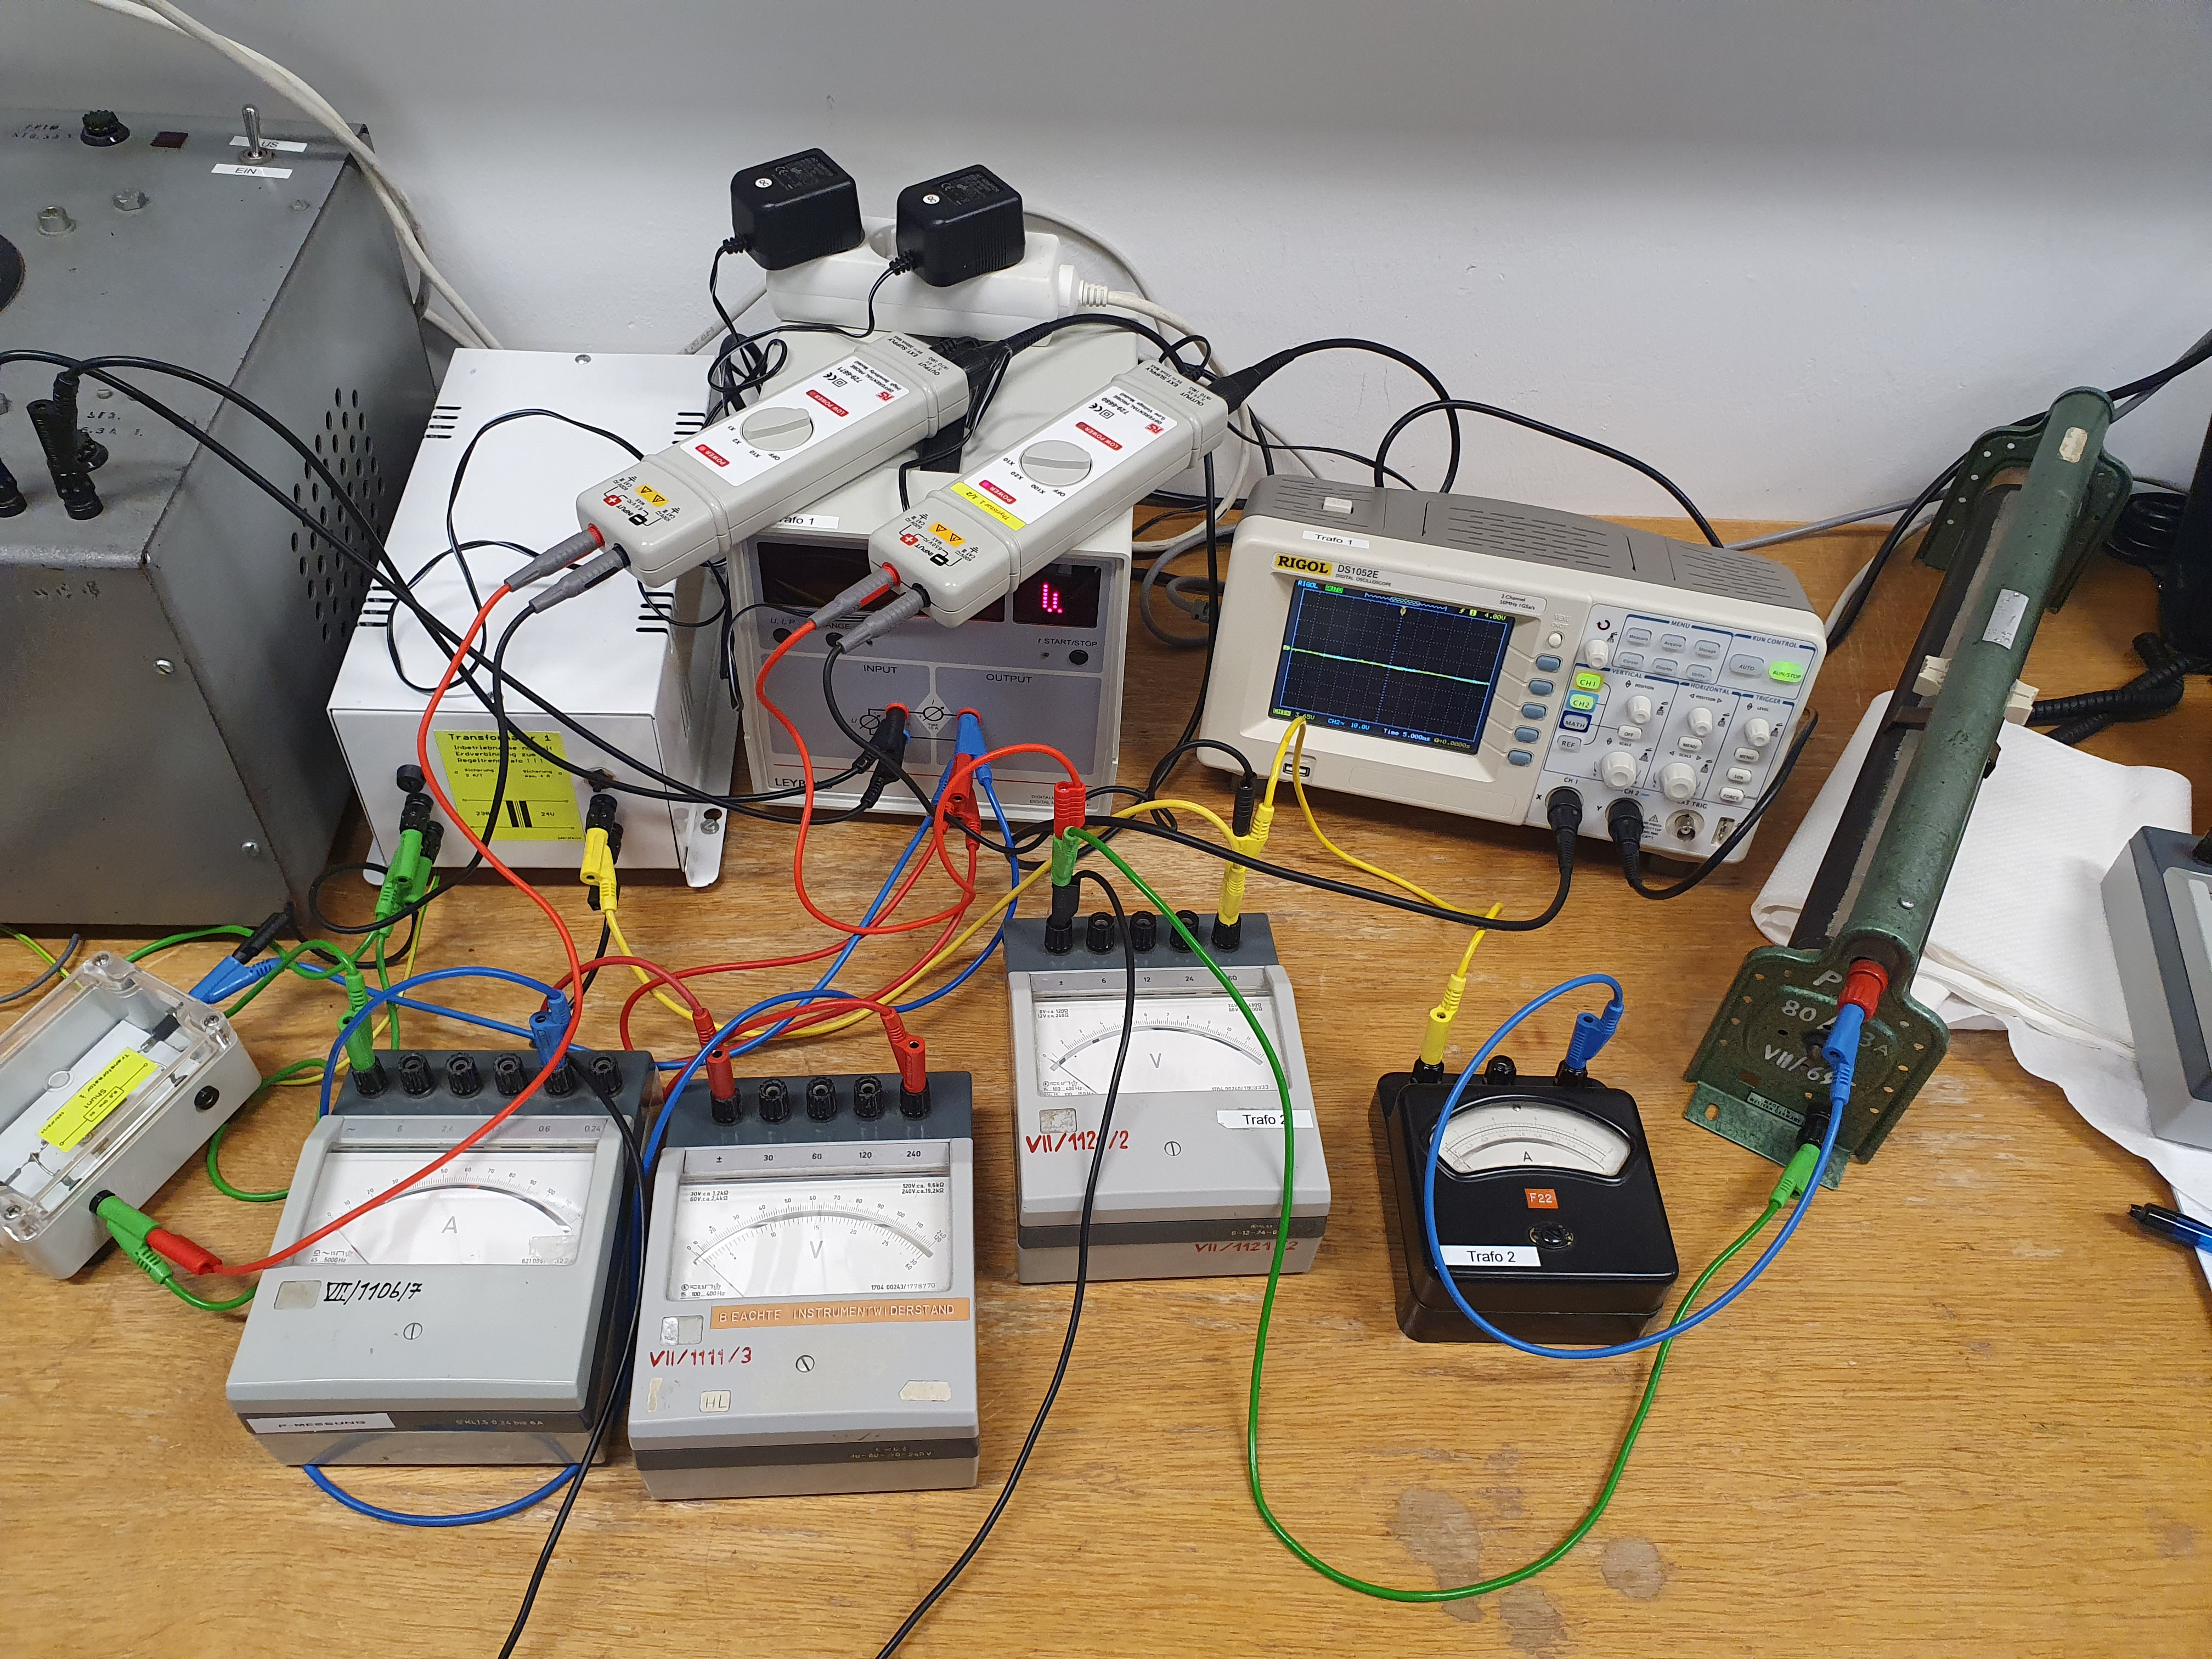
\includegraphics[width=0.6\linewidth, angle=0]{nudes/Aufbau b.png}
    \caption{Realer Aufbau mit Lastwiderstand}
    \label{fig:RealerAufbauB}
\end{figure}

\noindent
Für die letzte Erweiterung der Grundschaltung wurde nun noch eine Spule seriell an das Potentiometer angeschlossen. Weiters war nun ein weiteres Voltmeter zur Bestimmung der Spannung $U_{R}$, welche später für die Berechnung der Leistung $P_{2}$ noch benötigt wird.

\begin{figure}[H]
    \centering
    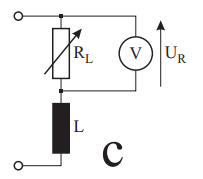
\includegraphics[width=0.2\linewidth, angle=0]{nudes/Versuchsaufbau c.png}
    \caption{Potentiometer und Spule als zusätzliche Verbraucher}
    \label{fig:AufbauB}
\end{figure}

\begin{figure}[H]
    \centering
    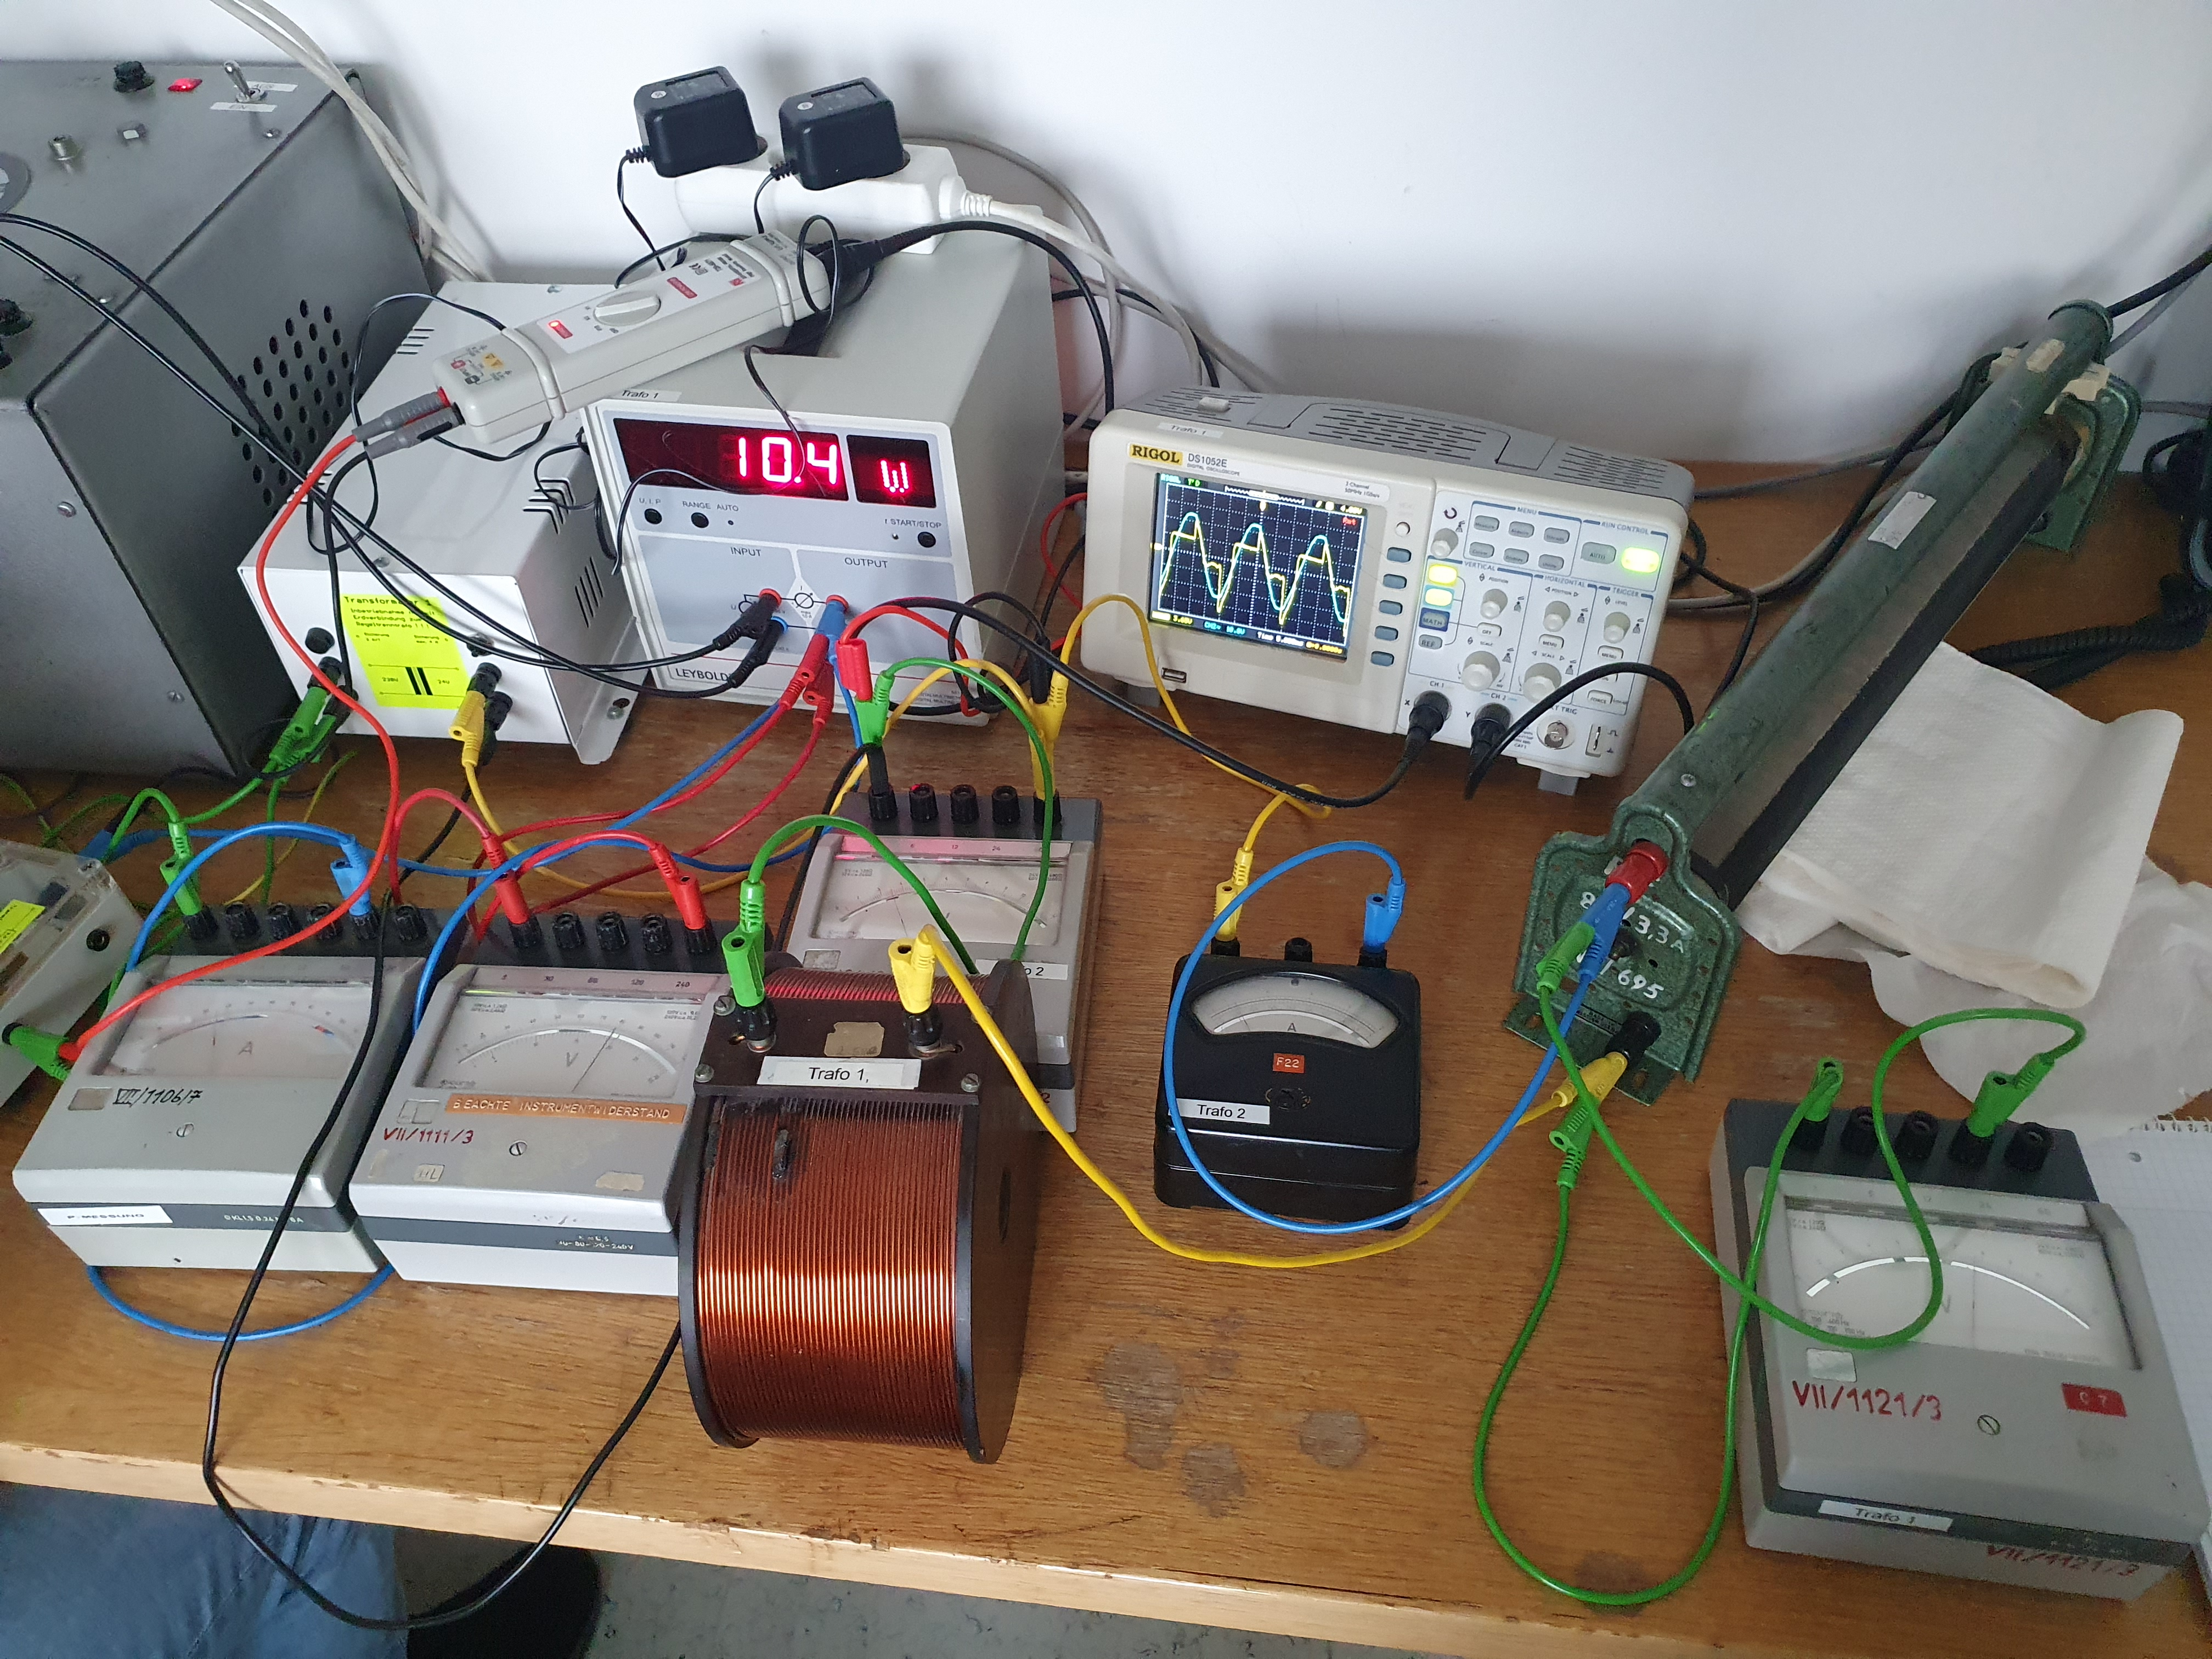
\includegraphics[width=0.6\linewidth, angle=0]{nudes/Aufbau c.png}
    \caption{Realer Aufbau mit Potentiometer und Spule}
    \label{fig:RealerAufbauB}
\end{figure}



\section{Geräteliste} %jo holt a listn ------------------------------

    \begin{table}[H]
        \centering
        \caption{Im Versuch verwendete Geräte und Utensilien.}
        \label{tab:geraete}
        \begin{tabular}{| l | l | l | l |}
            \hline
            Gerät & Gerätenummer  & Unsicherheit \\
            Oszilloskop & {n.a} & {n.a} \\
            Trafo Tr1 & {n.a} & {n.a} \\
            Trafo Tr2 & {n.a} & {n.a} \\
            Multimeter P & {n.a} & $\pm 0.001 W$ \\
            Potentiometer & {n.a} & {n.a} \\
            Shunt & {n.a} & {n.a} \\
            Voltmeter U1 & {n.a} & $\pm 0.5\%$ + 2 digit \\
            Voltmeter U2 & {n.a} & $\pm 0.5\%$ + 2 digit \\
            Voltmeter UR & {n.a} & $\pm 0.5\%$ + 2 digit \\
            Amperemeter I1 & {n.a} & $\pm 1.5\%$ + 2 digit \\
            Amperemeter I2 & {n.a} & $\pm 0.5\%$ + 2 digit \\
            Spule & {n.a} & {n.a} \\
            \hline
        \end{tabular}
    \end{table}


\section{Versuchsdurchführung \& Messergebnisse} %nachvollziehbar und klar dargestellt ------------------------------


\section{Auswertung und Unsicherheitsanalyse} %Nicht nur zahlen angeben ------------------------------

In der Auswertung werden zur erhöhten Genauigkeit durchgehend ungerundete Werte bis zu den Endergebnissen verwendet und nur zur Darstellung gerundet. \\
Zur Berechnung der Unsicherheiten wird, wenn nicht anders angegeben, die Größtunsicherheitsmethode verwendet.


\section{Diskussion} %diskussion der Unsicherheiten und Ergebnisse und evtl. verlgeich mit Literatur ------------------------------


\section{Zusammenfassung} %klare, übersichtliche vollständige beantwortung der Aufgabenstellung ------------------------------


\printbibliography[heading=bibintoc]
\end{document}
